
%(BEGIN_QUESTION)
% Copyright 2011, Tony R. Kuphaldt, released under the Creative Commons Attribution License (v 1.0)
% This means you may do almost anything with this work of mine, so long as you give me proper credit

Suppose you need to test a multi-pair electrical cable before it is used as part of a FOUNDATION Fieldbus H1 network.  The cable ends are terminated at terminal blocks too far away to permit a multimeter's test leads to stretch from one end to the other:

$$\includegraphics[width=15.5cm]{i00448x01.eps}$$

Devise a series of measurements that a technician could take using a multimeter located at one end of the cable.  Be sure to specify which setting the multimeter should be configured for, and which terminals the test leads should touch.  Also, be sure to specify what range of measurements would indicate ``good'' versus ``bad'' for each test:

\begin{itemize}
\item{} Pair ``B'' wires shorted together in cable
\vskip 10pt
\item{} Either conductor of Pair ``B'' being broken (open)
\vskip 10pt
\item{} Either conductor of Pair ``B'' shorted to cable shield
\vskip 10pt
\item{} Either conductor of Pair ``B'' shorted to either conductor of pair ``A''
\end{itemize}

\vskip 20pt \vbox{\hrule \hbox{\strut \vrule{} {\bf Suggestions for Socratic discussion} \vrule} \hrule}

\begin{itemize}
\item{} What purpose does the {\it shield} conductor serve in a multi-conductor cable?
\end{itemize}

\underbar{file i00448}
%(END_QUESTION)





%(BEGIN_ANSWER)

\noindent
{\bf Partial answer:}

\vskip 10pt

You must perform {\it continuity} tests using the multimeter set to its ``resistance'' (ohms) measuring function.  Low resistance indicates continuity, while high resistance indicates lack of continuity.

\vskip 10pt

The {\it real} question in each case is which terminals we must measure between with the multimeter in order to test for each possible cable fault!  This I leave to you to figure out.

%(END_ANSWER)





%(BEGIN_NOTES)

\begin{itemize}
\item{} Pair ``B'' wires shorted together in cable: {\it measure resistance between terminals 3 and 4.  High resistance is good, while low resistance indicates a short.}
\vskip 10pt
\item{} Either conductor of Pair ``B'' being broken (open): {\it short terminals 3 and 4 together at one end of the cable, then measure resistance between terminals 3 and 4 at the other end of the cable.  Low resistance is good, while high resistance indicates an open.}
\vskip 10pt
\item{} Either conductor of Pair ``B'' shorted to cable shield: {\it measure resistance between terminals 3 and 7, then between 4 and 7.  High resistance in either case is good, while low resistance in either case indicates a short.}
\vskip 10pt
\item{} Either conductor of Pair ``B'' shorted to either conductor of pair ``A'': {\it measure resistance between the following terminal pairs: 3 and 1, 3 and 2, 4 and 1, 4 and 2.  High resistance is good, while low resistance indicates a short.}
\end{itemize}

%INDEX% Electronics review: continuity-checking a multi-pair cable

%(END_NOTES)

